\documentclass[11pt]{article}
\usepackage[margin=1in]{geometry}
\usepackage{amsmath,amssymb,amsthm,mathtools}
\usepackage{booktabs}
\usepackage{float}
\usepackage{graphicx}
\usepackage[hidelinks]{hyperref}
\usepackage{microtype}

\newtheorem{theorem}{Theorem}
\newtheorem{lemma}[theorem]{Lemma}
\newtheorem{corollary}[theorem]{Corollary}
\theoremstyle{remark}
\newtheorem{remark}[theorem]{Remark}

\newcommand{\T}{\mathbb T}
\newcommand{\C}{\mathbb C}
\newcommand{\KR}{K_{\mathbb R}}
\newcommand{\KC}{K_{\mathbb C}}
\makeatletter
\renewcommand{\@seccntformat}[1]{\csname the#1\endcsname\hspace{0.8em}}
\makeatother

\title{Real and Complex Unconditional Constants\
Are Different for a Five-Character Basis}
\author{Candidate full affirmative answer to the final question in arXiv:0703236}
\date{13 August 2026}

\begin{document}
\maketitle

\begin{center}
\fbox{\parbox{0.92\linewidth}{\textbf{Status.}
Candidate full result, subject to human review.  For the explicit frequency
set $\Lambda=\{0,1,2,3,5\}$, a static interval certificate proves
\[
 \KC(\Lambda)>\frac{49999}{26400}>1.89>1.888>\KR(\Lambda).
\]
Thus the real and complex unconditional constants of a finite character
basis can differ.}}
\end{center}

\section{Question and current-status evidence}

For a finite $\Lambda\subset\mathbb Z$, let
\[
 C_\Lambda=\operatorname{span}\{e_\lambda:\lambda\in\Lambda\}
 \subset C(\T),\qquad e_\lambda(z)=z^\lambda,
\]
with the supremum norm.  Write $M_u(\sum c_\lambda e_\lambda)
=\sum u_\lambda c_\lambda e_\lambda$.  The real and complex unconditional
constants are
\[
 \KR(\Lambda)=\max_{u_\lambda\in\{-1,1\}}\|M_u\|,
 \qquad
 \KC(\Lambda)=\max_{|u_\lambda|=1}\|M_u\|.
\]

Neuwirth's source paper proves equality for every three-character basis and
ends by asking whether the constants can be different for larger finite sets
\cite{source}.  The exact source passage is reproduced below.

\begin{figure}[H]
  \centering
  
\includegraphics[width=0.80\textwidth]{figures/source_open_question.png}
  \caption{The open question in arXiv:0703236, PDF page 23.}
\end{figure}

A later posting by the same author computes the real constant for
$\{0,1,2,3\}$ but explicitly says the general distinction remains undecided
\cite{status}.  Its manuscript is dated 2013 and it was posted to arXiv in
2026.

\begin{figure}[H]
  \centering
  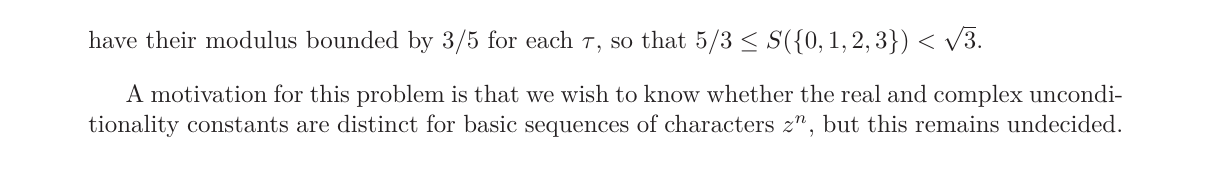
\includegraphics[width=0.92\textwidth]{figures/support_open_status.png}
  \caption{Later status evidence, arXiv:2603.28229, PDF page 1.}
\end{figure}

\section{The result}

\begin{theorem}\label{thm:gap}
For $\Lambda=\{0,1,2,3,5\}$,
\[
 \KC(\Lambda)>\frac{49999}{26400}>1.89
 \quad\text{and}\quad
 \KR(\Lambda)<1.888=\frac{236}{125}.
\]
In particular,
\[
 \KC(\Lambda)-\KR(\Lambda)>\frac{779}{132000}.
\]
\end{theorem}

The proof has an elementary reduction and two finite certificates.  All
certificate data and the outward-rounded checker are in
\texttt{code/verify\_gap.py}.

\section{Two norm reductions}

\begin{lemma}\label{lem:reductions}
For every finite $\Lambda$,
\begin{align*}
 \KC(\Lambda)
 &=\sup_{0\ne p=\sum c_\lambda z^\lambda}
   \frac{\sum_{\lambda\in\Lambda}|c_\lambda|}{\|p\|_\infty},\\
 \KR(\Lambda)
 &=\max_{\varepsilon\in\{-1,1\}^\Lambda}\|L_\varepsilon\|,
 \qquad
 L_\varepsilon\!\left(\sum c_\lambda z^\lambda\right)
 =\sum\varepsilon_\lambda c_\lambda.
\end{align*}
\end{lemma}

\begin{proof}
For the first identity, every complex multiplier satisfies
$|\sum u_\lambda c_\lambda z^\lambda|\leq\sum|c_\lambda|$.
Conversely, for fixed coefficients choose
$u_\lambda=\overline{c_\lambda}/|c_\lambda|$ (arbitrarily if
$c_\lambda=0$) and evaluate at $z=1$.

For the second identity, fix a sign pattern $\varepsilon$.  If $|\zeta|=1$
and $d_\lambda=c_\lambda\zeta^\lambda$, then
\[
 \left\|\sum d_\lambda z^\lambda\right\|_\infty
 =\left\|\sum c_\lambda z^\lambda\right\|_\infty,
 \qquad
 \sum\varepsilon_\lambda d_\lambda
 =(M_\varepsilon p)(\zeta).
\]
Taking the two suprema gives $\|M_\varepsilon\|=\|L_\varepsilon\|$.
\end{proof}

\section{The complex lower certificate}

Consider
\begin{align*}
 p(z)=\frac1{100000}\big(&19563+18666z+(-6125-28872i)z^2\\
                         &+(18692+10604i)z^3+(-5823+9055i)z^5\big).
\end{align*}
The three nonreal coefficient moduli have the exact integer brackets
\[
\begin{aligned}
29514^2&\leq871108009\leq29515^2,\\
21490^2&\leq461835680\leq21491^2,\\
10765^2&\leq115900354\leq10766^2.
\end{aligned}
\]
Consequently
\[
 \sum_{\lambda\in\Lambda}|c_\lambda|
 \geq\frac{19563+18666+29514+21490+10765}{100000}
 =\frac{99998}{100000},
\]
whereas the corresponding upper brackets give
\[
 \|p'\|_\infty
 \leq\sum\lambda|c_\lambda|
 <\frac{49}{25}.
\]

At each of the $4096$th roots of unity, outward-rounded interval evaluation
gives
\[
 \max_{0\leq k<4096}|p(e^{2\pi i k/4096})|
 <0.52631.
\]
Every point of $\T$ lies at angular distance at most $\pi/4096$ from this
grid.  The mean-value estimate and $\pi<22/7$ therefore yield
\[
 \|p\|_\infty
 <\frac{52631}{100000}
   +\frac{49}{25}\frac{22}{7\cdot4096}
 =\frac{3378009}{6400000}
 <\frac{66}{125}.
\]
Lemma~\ref{lem:reductions} now proves
\[
 \KC(\Lambda)>
 \frac{99998/100000}{66/125}=\frac{49999}{26400}.
\]

\section{The real upper certificate}

We use the following standard dual certificate.  If a finite complex measure
$\mu$ on $\T$ satisfies
\[
 \int_\T z^\lambda\,d\mu(z)=\varepsilon_\lambda
 \quad(\lambda\in\Lambda),
\]
then $L_\varepsilon(f)=\int f\,d\mu$ and hence
$\|L_\varepsilon\|\leq\|\mu\|_{\mathrm{TV}}$.

It suffices to take $\varepsilon_0=1$, since simultaneous sign reversal does
not change the norm.  For each of the resulting $16$ patterns, the checker
stores a measure $\nu$ whose atoms have the exact form
\[
 \frac{a}{10^{12}}e^{-2\pi i p/120}\,
 \delta_{e^{2\pi i t/120}},
 \qquad a,p,t\in\mathbb Z,\ a\geq0.
\]
Thus $\|\nu\|_{\mathrm{TV}}=\sum a/10^{12}$ exactly.  Its five moment
residuals are evaluated by outward-rounded interval arithmetic.

For completeness, the rounding residual is repaired analytically rather than
ignored.  Put
\[
 q_\lambda=\varepsilon_\lambda-\int z^\lambda\,d\nu(z)
 \quad(\lambda\in\Lambda),\qquad q_4=0,
\]
let $\omega=e^{2\pi i/6}$, and define
\[
 b_k=\frac16\sum_{j=0}^5q_j\omega^{-kj},\qquad
 \eta=\sum_{k=0}^5 b_k\delta_{\omega^k}.
\]
Discrete Fourier inversion gives
$\int z^j\,d\eta(z)=q_j$ for $0\leq j\leq5$, while
\[
 \|\eta\|_{\mathrm{TV}}
 \leq\sum_{j=0}^5|q_j|=\sum_{\lambda\in\Lambda}|q_\lambda|.
\]
Therefore $\mu=\nu+\eta$ is an exact representing measure and
\[
 \|L_\varepsilon\|
 \leq\|\nu\|_{\mathrm{TV}}
     +\sum_{\lambda\in\Lambda}|q_\lambda|.
\]

The following are decimal displays of rigorous interval upper bounds from the
static checker.  Each has been rounded upward to the shown sixth decimal.
\[
\begin{array}{c r@{\qquad}c r}
\toprule
\varepsilon&\text{bound}&\varepsilon&\text{bound}\\
\midrule
\texttt{+----}&1.872706&\texttt{+---+}&1.666667\\
\texttt{+--+-}&1.414214&\texttt{+--++}&1.751844\\
\texttt{+-+--}&1.000001&\texttt{+-+-+}&1.521691\\
\texttt{+-++-}&1.887888&\texttt{+-+++}&1.666667\\
\texttt{++---}&1.751844&\texttt{++--+}&1.414214\\
\texttt{++-+-}&1.666667&\texttt{++-++}&1.872706\\
\texttt{+++--}&1.666667&\texttt{+++-+}&1.887888\\
\texttt{++++-}&1.521691&\texttt{+++++}&1.000001\\
\bottomrule
\end{array}
\]
In particular, all $16$ exact corrected measures have total variation less
than $1.888$, so Lemma~\ref{lem:reductions} gives $\KR(\Lambda)<1.888$.

\begin{proof}[Proof of Theorem~\ref{thm:gap}]
The complex and real estimates were proved in the preceding two sections.
Finally,
\[
 \KC(\Lambda)-\KR(\Lambda)
 >\frac{49999}{26400}-\frac{236}{125}
 =\frac{779}{132000}>0.
\]
\end{proof}

\section{Verification and novelty assessment}

The checker contains no optimization call and no downloaded data: it consists
only of the displayed rational polynomial, the finite atom lists, exact
integer/rational arithmetic, and outward-rounded evaluations of roots of
unity using \texttt{mpmath.iv}.  It checks the coefficient brackets, the
$4096$ grid, the derivative correction, all $16$ normalized sign patterns,
the DFT residual bound, and the final rational gap.  A clean run prints
\begin{verbatim}
complex witness grid upper: 0.526309881899435
certified complex constant lower bound: 1.893901515151515
worst normalized real sign: +-++-
worst corrected real certificate: 1.887887419718339
CERTIFIED: K_C > 49999/26400 > 1.89 > 1.888 > K_R
certified gap lower bound: 779/132000
\end{verbatim}

The local run indexes and a bounded arXiv/web search on 13 August 2026 found
no prior example separating the two constants.  The later same-author status
paper still calls the distinction undecided.  The construction and constants
above should therefore be treated as a new candidate full answer, with high
correctness confidence from the static certificate and moderate-to-high
novelty confidence pending specialist review.

\begin{thebibliography}{9}
\bibitem{source}
S.~Neuwirth,
\emph{The maximum modulus of a trigonometric trinomial},
arXiv:math/0703236 (2007; revised 2008).

\bibitem{status}
S.~Neuwirth,
\emph{On the (Fourier analytic) Sidon constant of $\{0,1,2,3\}$},
arXiv:2603.28229 (posted 2026; manuscript dated 2013).
\end{thebibliography}

\end{document}
